\subsection{Alternative Scheme}

Now that the CPPI model is presented and its logic understood, we can move upon to alternatives. One of the main characteristics of the CPPI model is that it is defined thanks to a constant, invariant $\pi$ that settles the risk exposure of the investor. An interesting approach would not just change this parameter, but make it \emph{variable}.

Normally, the simplest approach to ensure that an investment has a defined and controlled risk profile is to set a $\pi$ constant proportion of the investment to be allocated in risky assets, as done in the CPPI. That proportion is defined by the risk aversion profile of the investor, but is invariable throughout the investment.

However, the work of \cite{a:guillen-optimisation} showed that, given some investment plan ending at time $T$ with $X(T)$ final wealth, risk aversion profile defined by $\gamma$ and a maximum possible allowed loss $K$, we can set the utility function

\begin{align}
    u_\gamma = \frac{1}{\gamma}\qty(X(T) + K)^\gamma \emph{.}
\end{align}

Whose expected value for any given present wealth $x = X(t)$ is defined as

\begin{align}\label{eq:maxE}
    \max_{\pi}\EX\giventhat{u_{X(T)}}{x} \emph{,}
\end{align}

which can be maximized~\cite{a:guillen-optimisation} by a strategy that invests a relative amount in risky assets variable at any time $t \in [0,T)$, whose solution is:

\begin{align}\label{eq:the_formula}
    \pi(t)X(t) = A\qty(K + X(t) + g(t)) \textit{.}
\end{align}

Where $X(t)$ is the wealth at time $t$, $A$ is a parameter that defines the risk aversion profile of the investor, $K$ is the maximum loss the investor is capable to handle and $g(t)$ is the sum of all remaining inputs or outputs of money~\footnote{In \cite{a:donnelly-savings-decisions}'s work, the authors defined optimal savings strategies and analysed different updating periods for $\pi$.}: $g(t) = \sum_{i=t}^{T}a_i$. Thus, the time evolution of the wealth $X$ of an investor would behave as following:

\begin{align}
    dX = \alpha \pi(t)X(t)dt + \sigma \pi(t)X(t)dW(t) + dC(t)\textit{.}
\end{align}

Where $\alpha$ is the expected return of the risky market, $\sigma$ is the expected volatility of the risky market, $W(t)$ is a Wiener process and $C(t)$ is the allocated or consumed capital by the investor at every time step.

\subsection*{Simulation}

In order to analyse the alternative scheme, the process will be quite similar to the previous one. We set the normal behaviour of the price evolution of the risky asset, and fix all parameters. Thus, the wealth of the investor behaves as follows:

\begin{align}
    X_{t+1} = \qty(1+N(\alpha, \sigma))X_t \pi_t + \qty(1 - \pi_t)X_t + C(t) \textit{,}
\end{align}

where

\begin{align}
    \pi_t = \frac{A\qty(K + X_T + \sum_t^T C(t))}{X_T} \quad \textit{and}
\end{align}

\begin{equation*}
    C(t) =
    \begin{cases*}
      a & if $t <= T/2$ \\
      -a       & if $t > T/2$ \textit{.}
    \end{cases*}
\end{equation*}

Again, at the end of all $T$ years, the final wealth $X_T$ remaining to the saver it is stored, and then all the process is repeated. This way we manage to compute tens of thousands of different performances and make some statistics out of them.

\begin{figure}[H]
    \centering
    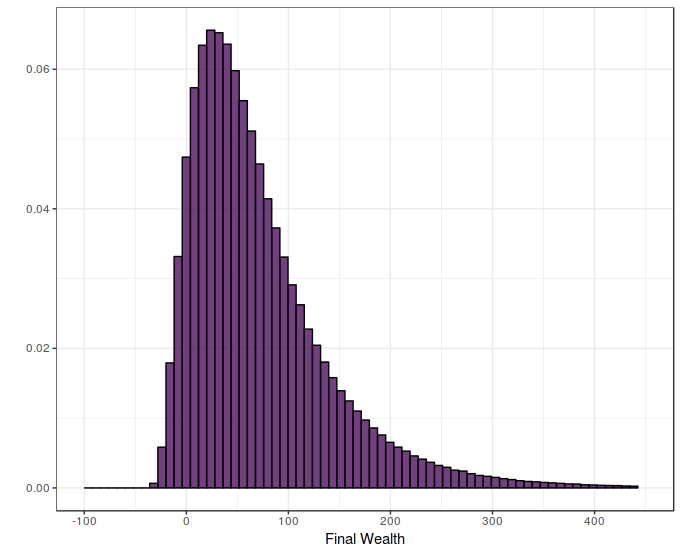
\includegraphics[scale=0.65]{./images/fw_alt.png}
    \caption{Results of $100,000$ simulations for the \textit{Alternative} model. Final wealth obtained for every simulation, where $T=30$, $\mu = 0.0343$, $\sigma = 0.1544$, $a=10$, $\pi = 0.1$.}
    \label{fig:alt_fw}
\end{figure}

In the case of figure \ref{fig:alt_fw}, where the right tail corresponds to large values of wealth, whereas the left part deals with losses; we can see how outrageously obvious is that it does \textit{not} follow a Normal Distribution.

The code necessary to replicate these results in R can be found in Appendix \ref{ap:alt-simple}.
